\begin{figure}[tb]
\centering
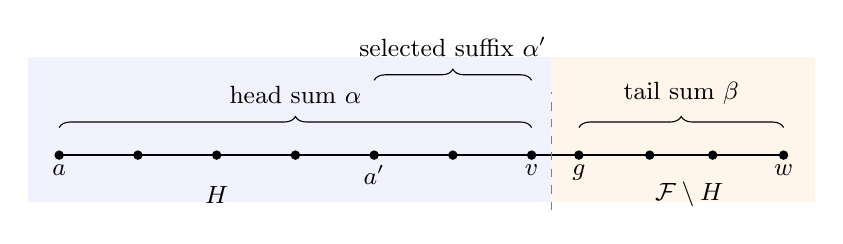
\begin{tikzpicture}[x=1cm,y=1cm,font=\small]
 \fill[blue!5] (-.4,-.6) rectangle (6.25,1.25);
 \fill[orange!8] (6.25,-.6) rectangle (9.6,1.25);
 \draw[thick] (0,0)--(9.2,0);
 \draw[dashed,gray] (6.25,-.7)--(6.25,.8);
 \foreach \x in {0,1,2,3,4,5,6,6.6,7.5,8.3,9.2}
   \fill (\x,0) circle (1.7pt);
 \node[below] at (0,0) {$a$};
 \node[below] at (4,0) {$a'$};
 \node[below] at (6,0) {$v$};
 \node[below] at (6.6,0) {$g$};
 \node[below] at (9.2,0) {$w$};
 \draw[decorate,decoration={brace,amplitude=4pt}] (0,.35)--(6,.35)
   node[midway,above=5pt] {head sum $\alpha$};
 \draw[decorate,decoration={brace,amplitude=4pt}] (4,.95)--(6,.95)
   node[midway,above=5pt] {selected suffix $\alpha'$};
 \draw[decorate,decoration={brace,amplitude=4pt}] (6.6,.35)--(9.2,.35)
   node[midway,above=5pt] {tail sum $\beta$};
 \node at (2,-.5) {$H$};
 \node at (8,-.5) {$\mathcal F\setminus H$};
\end{tikzpicture}
\caption{The threshold cut for a crossing segment. Its head has
$f$-sum $\alpha$ and its selected suffix has $f$-sum $\alpha'$.
When $\alpha\beta>0$ and $|\alpha|>2sm_g$, the sign choice gives
$\alpha\alpha'<0$ and $|\alpha'|\ge2sm_g$.
Cutting immediately before $a'$ therefore increases the squared
$f$-test by at least $2s\alpha\beta$. The vertex spacing is schematic.}
\label{fig:paired-cut}
\end{figure}
